\documentclass[10pt, aspectratio=169]{beamer}
\usetheme[progressbar=frametitle, block=fill]{metropolis}

\usepackage{booktabs}
\usepackage{xcolor}
\usepackage{colortbl}
\usepackage{tikz}
\usetikzlibrary{positioning}
\usepackage{pgfplots}
\pgfplotsset{compat=1.18}

% Colors
\definecolor{lovecraftred}{RGB}{180,40,40}
\definecolor{highchi}{RGB}{160,60,60}
\definecolor{midchi}{RGB}{100,100,160}
\definecolor{lowchi}{RGB}{50,120,80}
\definecolor{accent}{RGB}{83,74,183}
\definecolor{axisweight2}{RGB}{220,230,255}

\setbeamercolor{frametitle}{bg=black, fg=white}
\setbeamercolor{progress bar}{fg=accent}
\setbeamercolor{alerted text}{fg=lovecraftred}

\title{The Cosmic Horror Index}
\subtitle{Rating Every Cosmology on the Lovecraft Scale}
\author{Seckin Ozbek}
\date{}

% ---------------------------------------------------------------
\begin{document}

% ---- SLIDE 1: TITLE -------------------------------------------
\maketitle

% ---- SLIDE 2: THE QUESTION ------------------------------------
\begin{frame}{The Question}
  \vspace{1em}
  \begin{center}
    \large
    \textit{Does the universe care about you?}\\[1.2em]
    \textbf{\Large Most traditions say no.}\\[1.8em]
    \normalsize
    But \textit{how much} they don't care — and \textit{why} — varies dramatically.\\[0.8em]
    The Cosmic Horror Index measures that variance\\
    from textual evidence, not intuition.
  \end{center}
\end{frame}

% ---- SLIDE 3: THE 10 AXES -------------------------------------
\begin{frame}{The 10 Axes}
  \small
  \begin{center}
  \begin{tabular}{lll}
    \toprule
    \textbf{Axis} & \textbf{High score} & \textbf{Wt} \\
    \midrule
    \rowcolor{axisweight2}
    Indifference to humans       & Universe doesn't notice us    & \textbf{2$\times$} \\
    \rowcolor{axisweight2}
    Incomprehensibility          & Reality breaks minds          & \textbf{2$\times$} \\
    \rowcolor{axisweight2}
    Human insignificance         & We are cosmically irrelevant  & \textbf{2$\times$} \\
    Omniscience                  & All-knowing ultimate reality  & 1 \\
    Omnipotence                  & Absolute, unchallengeable power & 1 \\
    Self-sufficiency             & Needs nothing from creation   & 1 \\
    Cyclical destruction         & Cosmos destroys and rebuilds  & 1 \\
    Awe / madness induction      & Truth is unbearable           & 1 \\
    Creation without consent     & Existence imposed on beings   & 1 \\
    Moral neutrality             & Beyond good and evil          & 1 \\
    \bottomrule
  \end{tabular}
  \end{center}
  \vspace{0.3em}
  \small\textcolor{accent}{Shaded axes carry 2$\times$ weight — they are Lovecraft's signature.}
\end{frame}

% ---- SLIDE 4: THE FORMULA -------------------------------------
\begin{frame}{The Formula}
  \vspace{0.5em}
  \textbf{CHI score} = weighted mean of 10 axis scores, each on $[0, 100]$:

  \vspace{0.8em}
  \[
    \mathrm{CHI} = \frac{2 \cdot S_\text{indiff} + 2 \cdot S_\text{incomp} + 2 \cdot S_\text{insignif}
                        + \sum_{\text{7 others}} S_i}{13}
  \]

  \vspace{0.8em}
  \textbf{Each axis score} from passage-level LLM classifications:
  \begin{itemize}
    \item Retrieve top-20 passages per (tradition, axis) via FAISS semantic search
    \item Claude scores each: \textit{relevance} $\in[0,1]$, \textit{valence} $\in[-1,+1]$, \textit{confidence} $\in[0,1]$
    \item Axis score $= \bar{v}_\text{weighted} \times 50 + 50$, where weights $= \text{rel} \times \text{conf}$
    \item 95\% CI from 1000-iteration bootstrap
  \end{itemize}

  \vspace{0.5em}
  \alert{Every score is traceable to specific passages.}
\end{frame}

% ---- SLIDE 5: NLP PIPELINE ------------------------------------
\begin{frame}{NLP Pipeline}
  \begin{center}
  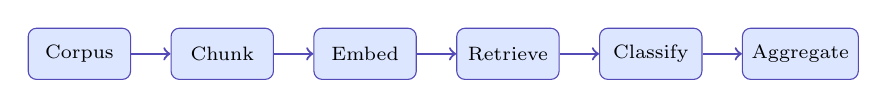
\begin{tikzpicture}[
    node distance=0.5cm,
    box/.style={rectangle, rounded corners=3pt, draw=accent, fill=axisweight2,
                minimum width=1.3cm, minimum height=0.65cm, font=\scriptsize, align=center},
    arr/.style={->, thick, color=accent}
  ]
    \node[box] (corpus)   {Corpus};
    \node[box] (chunk)    [right=of corpus]  {Chunk};
    \node[box] (embed)    [right=of chunk]   {Embed};
    \node[box] (retrieve) [right=of embed]   {Retrieve};
    \node[box] (classify) [right=of retrieve]{Classify};
    \node[box] (agg)      [right=of classify]{Aggregate};

    \draw[arr] (corpus)   -- (chunk);
    \draw[arr] (chunk)    -- (embed);
    \draw[arr] (embed)    -- (retrieve);
    \draw[arr] (retrieve) -- (classify);
    \draw[arr] (classify) -- (agg);
  \end{tikzpicture}
  \end{center}

  \vspace{0.6em}
  \begin{columns}[T]
    \column{0.33\textwidth}
      \textbf{Retrieval}\\
      Probe queries per axis\\
      Dynamic overfetch\\
      for small traditions
    \column{0.33\textwidth}
      \textbf{Classification}\\
      Structured JSON output\\
      Relevance gates passage\\
      min threshold = 0.2
    \column{0.33\textwidth}
      \textbf{Cost}\\
      \$9.40 full run\\
      \$0.72 / tradition\\
      $\sim$2 hr on CPU
  \end{columns}
\end{frame}

% ---- SLIDE 6: CORPUS ------------------------------------------
\begin{frame}{Corpus}
  \begin{columns}[T]
    \column{0.5\textwidth}
      \textbf{Scale}\\[0.4em]
      13 cosmological traditions\\
      14,096 text chunks\\
      all public domain (pre-1928)\\[0.8em]
      \textbf{Sources}\\[0.4em]
      Project Gutenberg (primary)\\
      AccessToInsight (Buddhism)\\
      gnosis.org (Gnosticism)\\
      sacred-texts.com
    \column{0.5\textwidth}
      \textbf{Traditions}\\[0.4em]
      Lovecraft \textbullet{} Absurdism \textbullet{} Daoism\\
      Gnosticism \textbullet{} Pantheism \textbullet{} Norse\\
      Bhakti Hinduism \textbullet{} Advaita Vedanta\\
      Aztec \textbullet{} Shinto \textbullet{} Greek\\
      Egyptian \textbullet{} Buddhism\\[0.8em]
      \textbf{Validation}\\[0.4em]
      Keyword check after every download\\
      7 wrong PG IDs caught \& corrected
  \end{columns}
\end{frame}

% ---- SLIDE 7: RESULTS -----------------------------------------
\begin{frame}{Results}
  \small
  \begin{columns}[T]
    \column{0.5\textwidth}
    \begin{tabular}{rlr}
      \toprule
      \# & Tradition & CHI \\
      \midrule
      \rowcolor{lovecraftred!20}
      1 & Lovecraft          & \textbf{73.6} \\
      \rowcolor{highchi!15}
      2 & Absurdism          & 64.6 \\
      \rowcolor{highchi!10}
      3 & Daoism             & 60.3 \\
      4 & Gnosticism         & 59.0 \\
      5 & Pantheism          & 56.0 \\
      6 & Norse              & 55.8 \\
      \bottomrule
    \end{tabular}
    \column{0.5\textwidth}
    \begin{tabular}{rlr}
      \toprule
      \# & Tradition & CHI \\
      \midrule
      7  & Bhakti Hinduism    & 55.2 \\
      8  & Advaita Vedanta    & 54.5 \\
      9  & Aztec              & 53.2 \\
      \rowcolor{lowchi!15}
      10 & Shinto             & 46.7 \\
      \rowcolor{lowchi!15}
      11 & Greek              & 46.3 \\
      \rowcolor{lowchi!20}
      12 & Egyptian           & 40.9 \\
      \rowcolor{lowchi!20}
      13 & Buddhism           & \textbf{40.8} \\
      \bottomrule
    \end{tabular}
  \end{columns}
  \vspace{0.4em}
  \small\textcolor{accent}{Lovecraft is the calibration anchor. Buddhism is the low anchor.}
\end{frame}

% ---- SLIDE 8: FINDING 1 ----------------------------------------
\begin{frame}{Finding 1: Most Cosmologies Lean Cosmic Horror}
  \vspace{0.5em}
  \begin{center}
  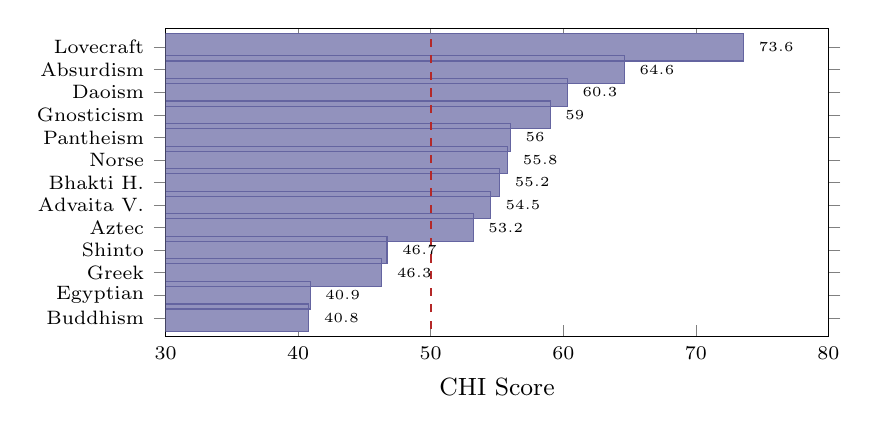
\begin{tikzpicture}
    \begin{axis}[
      xbar,
      width=10cm, height=5.5cm,
      xmin=30, xmax=80,
      ytick=data,
      yticklabels={Buddhism, Egyptian, Greek, Shinto, Aztec, Advaita V., Bhakti H.,
                   Norse, Pantheism, Gnosticism, Daoism, Absurdism, Lovecraft},
      yticklabel style={font=\scriptsize},
      xlabel={CHI Score},
      xlabel style={font=\small},
      xtick={30,40,50,60,70,80},
      xticklabel style={font=\scriptsize},
      bar width=0.35cm,
      enlarge y limits=0.07,
      nodes near coords,
      nodes near coords style={font=\tiny, xshift=2pt},
      every axis/.append style={font=\small},
    ]
      \addplot[fill=midchi!70, draw=midchi] coordinates {
        (40.8,0)(40.9,1)(46.3,2)(46.7,3)(53.2,4)
        (54.5,5)(55.2,6)(55.8,7)(56.0,8)(59.0,9)
        (60.3,10)(64.6,11)(73.6,12)
      };
      \draw[dashed, color=lovecraftred, line width=0.8pt] (axis cs:50,{-0.5}) -- (axis cs:50,{12.5})
        node[above, font=\tiny, color=lovecraftred] {50};
    \end{axis}
  \end{tikzpicture}
  \end{center}
  \small 10 of 13 traditions score above 50. The universe's indifference is a near-universal insight.
\end{frame}

% ---- SLIDE 9: FINDING 2 ----------------------------------------
\begin{frame}{Finding 2: Three Phases of Cosmological Horror}
  \vspace{0.6em}
  \begin{columns}[T]
    \column{0.33\textwidth}
      \textbf{\textcolor{lowchi}{Phase 1: Ancient}}\\[0.3em]
      \small
      Egyptian, Greek, Buddhist\\[0.2em]
      CHI: 41--46\\[0.2em]
      Gods are \textit{involved} —\\
      they judge, reward,\\
      and punish humans.\\[0.2em]
      Humans matter.
    \column{0.33\textwidth}
      \textbf{\textcolor{midchi}{Phase 2: Lovecraft}}\\[0.3em]
      \small
      Norse, Daoism,\\
      Gnosticism, Absurdism\\[0.2em]
      CHI: 55--73\\[0.2em]
      Indifference becomes\\
      explicit. Cosmos is\\
      vast and uncaring.\\[0.2em]
      \textit{We never mattered.}
    \column{0.33\textwidth}
      \textbf{\textcolor{lovecraftred}{Phase 3: New Weird}}\\[0.3em]
      \small
      VanderMeer,\\
      Ligotti, Watts\\[0.2em]
      CHI: 80+\,\textit{(est.)}\\[0.2em]
      Horror is the\\
      \textit{default} state.\\
      Consciousness is\\
      the aberration.\\[0.2em]
      \textit{Not yet scored.}
  \end{columns}
\end{frame}

% ---- SLIDE 10: REPO / HOW TO ----------------------------------
\begin{frame}{Open Dataset}
  \begin{columns}[T]
    \column{0.55\textwidth}
      \textbf{Repo}\\
      \small\texttt{github.com/seckinozbek1/cosmic-horror-index}\\[0.8em]
      \textbf{What's included}\\[0.3em]
      \small
      \texttt{output/chi\_dataset\_grounded.json}\\
      \quad All 13 traditions, 10 axes, bootstrap CIs\\[0.3em]
      \texttt{output/evidence\_document.md}\\
      \quad Every score traced to specific passages\\[0.3em]
      \texttt{config/pipeline\_config.yaml}\\
      \quad Axes, probes, corpus sources\\[0.8em]
      \textbf{Interactive viz}\\
      \small\texttt{seckinozbek1.github.io/cosmic-horror-index/}

    \column{0.45\textwidth}
      \textbf{Adding a tradition}\\[0.4em]
      \small
      1. Find public domain text (PG)\\
      2. Verify PG ID (never guess)\\
      3. Add to \texttt{pipeline\_config.yaml}\\
      4. \texttt{python tasks.py corpus <name>}\\
      5. \texttt{python tasks.py validate-corpus}\\
      6. \texttt{python tasks.py embed}\\
      7. \texttt{python tasks.py score <name>}\\[0.8em]
      \textbf{Cost: \$0.72 per tradition}\\
      \small See \texttt{docs/ADDING\_A\_TRADITION.md}
  \end{columns}
\end{frame}

\end{document}
